% Options for packages loaded elsewhere
\PassOptionsToPackage{unicode}{hyperref}
\PassOptionsToPackage{hyphens}{url}
%
\documentclass[
]{article}
\usepackage{lmodern}
\usepackage{amssymb,amsmath}
\usepackage{ifxetex,ifluatex}
\ifnum 0\ifxetex 1\fi\ifluatex 1\fi=0 % if pdftex
  \usepackage[T1]{fontenc}
  \usepackage[utf8]{inputenc}
  \usepackage{textcomp} % provide euro and other symbols
\else % if luatex or xetex
  \usepackage{unicode-math}
  \defaultfontfeatures{Scale=MatchLowercase}
  \defaultfontfeatures[\rmfamily]{Ligatures=TeX,Scale=1}
\fi
% Use upquote if available, for straight quotes in verbatim environments
\IfFileExists{upquote.sty}{\usepackage{upquote}}{}
\IfFileExists{microtype.sty}{% use microtype if available
  \usepackage[]{microtype}
  \UseMicrotypeSet[protrusion]{basicmath} % disable protrusion for tt fonts
}{}
\makeatletter
\@ifundefined{KOMAClassName}{% if non-KOMA class
  \IfFileExists{parskip.sty}{%
    \usepackage{parskip}
  }{% else
    \setlength{\parindent}{0pt}
    \setlength{\parskip}{6pt plus 2pt minus 1pt}}
}{% if KOMA class
  \KOMAoptions{parskip=half}}
\makeatother
\usepackage{xcolor}
\IfFileExists{xurl.sty}{\usepackage{xurl}}{} % add URL line breaks if available
\IfFileExists{bookmark.sty}{\usepackage{bookmark}}{\usepackage{hyperref}}
\hypersetup{
  pdftitle={STAT 626 Project},
  pdfauthor={Group 9},
  hidelinks,
  pdfcreator={LaTeX via pandoc}}
\urlstyle{same} % disable monospaced font for URLs
\usepackage[margin=1in]{geometry}
\usepackage{color}
\usepackage{fancyvrb}
\newcommand{\VerbBar}{|}
\newcommand{\VERB}{\Verb[commandchars=\\\{\}]}
\DefineVerbatimEnvironment{Highlighting}{Verbatim}{commandchars=\\\{\}}
% Add ',fontsize=\small' for more characters per line
\usepackage{framed}
\definecolor{shadecolor}{RGB}{248,248,248}
\newenvironment{Shaded}{\begin{snugshade}}{\end{snugshade}}
\newcommand{\AlertTok}[1]{\textcolor[rgb]{0.94,0.16,0.16}{#1}}
\newcommand{\AnnotationTok}[1]{\textcolor[rgb]{0.56,0.35,0.01}{\textbf{\textit{#1}}}}
\newcommand{\AttributeTok}[1]{\textcolor[rgb]{0.77,0.63,0.00}{#1}}
\newcommand{\BaseNTok}[1]{\textcolor[rgb]{0.00,0.00,0.81}{#1}}
\newcommand{\BuiltInTok}[1]{#1}
\newcommand{\CharTok}[1]{\textcolor[rgb]{0.31,0.60,0.02}{#1}}
\newcommand{\CommentTok}[1]{\textcolor[rgb]{0.56,0.35,0.01}{\textit{#1}}}
\newcommand{\CommentVarTok}[1]{\textcolor[rgb]{0.56,0.35,0.01}{\textbf{\textit{#1}}}}
\newcommand{\ConstantTok}[1]{\textcolor[rgb]{0.00,0.00,0.00}{#1}}
\newcommand{\ControlFlowTok}[1]{\textcolor[rgb]{0.13,0.29,0.53}{\textbf{#1}}}
\newcommand{\DataTypeTok}[1]{\textcolor[rgb]{0.13,0.29,0.53}{#1}}
\newcommand{\DecValTok}[1]{\textcolor[rgb]{0.00,0.00,0.81}{#1}}
\newcommand{\DocumentationTok}[1]{\textcolor[rgb]{0.56,0.35,0.01}{\textbf{\textit{#1}}}}
\newcommand{\ErrorTok}[1]{\textcolor[rgb]{0.64,0.00,0.00}{\textbf{#1}}}
\newcommand{\ExtensionTok}[1]{#1}
\newcommand{\FloatTok}[1]{\textcolor[rgb]{0.00,0.00,0.81}{#1}}
\newcommand{\FunctionTok}[1]{\textcolor[rgb]{0.00,0.00,0.00}{#1}}
\newcommand{\ImportTok}[1]{#1}
\newcommand{\InformationTok}[1]{\textcolor[rgb]{0.56,0.35,0.01}{\textbf{\textit{#1}}}}
\newcommand{\KeywordTok}[1]{\textcolor[rgb]{0.13,0.29,0.53}{\textbf{#1}}}
\newcommand{\NormalTok}[1]{#1}
\newcommand{\OperatorTok}[1]{\textcolor[rgb]{0.81,0.36,0.00}{\textbf{#1}}}
\newcommand{\OtherTok}[1]{\textcolor[rgb]{0.56,0.35,0.01}{#1}}
\newcommand{\PreprocessorTok}[1]{\textcolor[rgb]{0.56,0.35,0.01}{\textit{#1}}}
\newcommand{\RegionMarkerTok}[1]{#1}
\newcommand{\SpecialCharTok}[1]{\textcolor[rgb]{0.00,0.00,0.00}{#1}}
\newcommand{\SpecialStringTok}[1]{\textcolor[rgb]{0.31,0.60,0.02}{#1}}
\newcommand{\StringTok}[1]{\textcolor[rgb]{0.31,0.60,0.02}{#1}}
\newcommand{\VariableTok}[1]{\textcolor[rgb]{0.00,0.00,0.00}{#1}}
\newcommand{\VerbatimStringTok}[1]{\textcolor[rgb]{0.31,0.60,0.02}{#1}}
\newcommand{\WarningTok}[1]{\textcolor[rgb]{0.56,0.35,0.01}{\textbf{\textit{#1}}}}
\usepackage{graphicx,grffile}
\makeatletter
\def\maxwidth{\ifdim\Gin@nat@width>\linewidth\linewidth\else\Gin@nat@width\fi}
\def\maxheight{\ifdim\Gin@nat@height>\textheight\textheight\else\Gin@nat@height\fi}
\makeatother
% Scale images if necessary, so that they will not overflow the page
% margins by default, and it is still possible to overwrite the defaults
% using explicit options in \includegraphics[width, height, ...]{}
\setkeys{Gin}{width=\maxwidth,height=\maxheight,keepaspectratio}
% Set default figure placement to htbp
\makeatletter
\def\fps@figure{htbp}
\makeatother
\setlength{\emergencystretch}{3em} % prevent overfull lines
\providecommand{\tightlist}{%
  \setlength{\itemsep}{0pt}\setlength{\parskip}{0pt}}
\setcounter{secnumdepth}{-\maxdimen} % remove section numbering
\usepackage[]{natbib}
\bibliographystyle{plainnat}

\title{STAT 626 Project}
\author{Group 9}
\date{6/2021 - 8/2021}

\begin{document}
\maketitle

\begin{Shaded}
\begin{Highlighting}[]
\KeywordTok{library}\NormalTok{(astsa)}
\NormalTok{raw <-}\StringTok{ }\KeywordTok{read.csv}\NormalTok{(}\StringTok{"mlb.csv"}\NormalTok{)}
\NormalTok{era <-}\StringTok{ }\KeywordTok{ts}\NormalTok{(}\KeywordTok{rev}\NormalTok{(raw}\OperatorTok{$}\NormalTok{ERA), }\DataTypeTok{start =}\NormalTok{ raw}\OperatorTok{$}\NormalTok{Year[}\KeywordTok{length}\NormalTok{(raw}\OperatorTok{$}\NormalTok{Year)], }\DataTypeTok{end =}\NormalTok{ raw}\OperatorTok{$}\NormalTok{Year[}\DecValTok{1}\NormalTok{])}
\KeywordTok{tsplot}\NormalTok{(era, }\DataTypeTok{main =} \StringTok{'Earned Run Average Time Series'}\NormalTok{, }\DataTypeTok{xlab =} \StringTok{'Year'}\NormalTok{, }\DataTypeTok{ylab =} \StringTok{'ERA'}\NormalTok{)}
\end{Highlighting}
\end{Shaded}

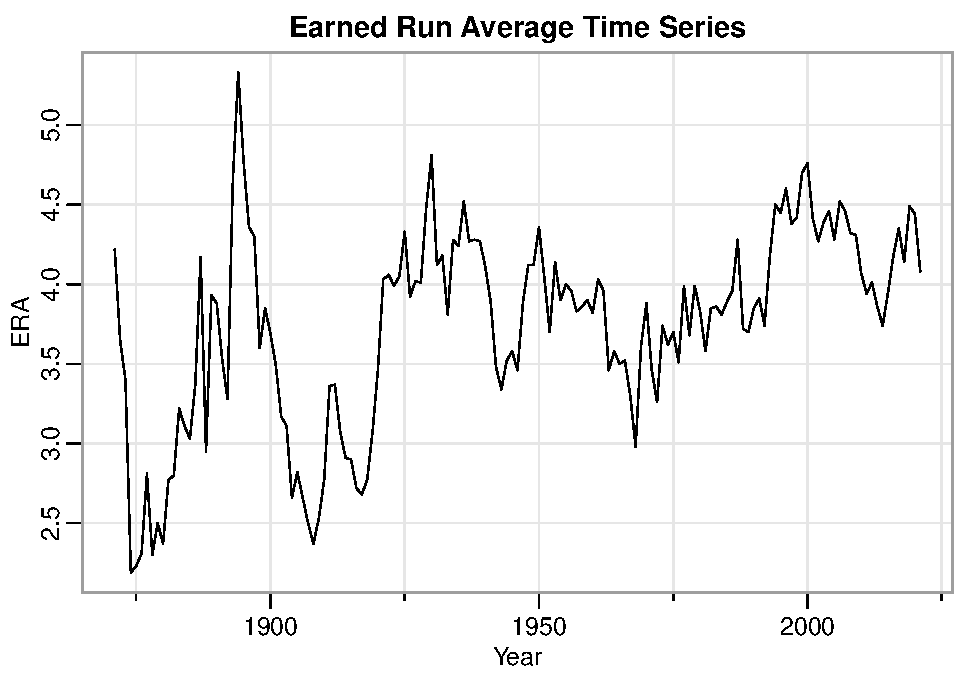
\includegraphics{project_files/figure-latex/unnamed-chunk-1-1.pdf}

\begin{Shaded}
\begin{Highlighting}[]
\NormalTok{ba <-}\StringTok{ }\KeywordTok{ts}\NormalTok{(}\KeywordTok{rev}\NormalTok{(raw}\OperatorTok{$}\NormalTok{BA), }\DataTypeTok{start =}\NormalTok{ raw}\OperatorTok{$}\NormalTok{Year[}\KeywordTok{length}\NormalTok{(raw}\OperatorTok{$}\NormalTok{Year)], }\DataTypeTok{end =}\NormalTok{ raw}\OperatorTok{$}\NormalTok{Year[}\DecValTok{1}\NormalTok{])}
\KeywordTok{tsplot}\NormalTok{(ba, }\DataTypeTok{main =} \StringTok{'Batting Average Time Series'}\NormalTok{, }\DataTypeTok{xlab =} \StringTok{'Year'}\NormalTok{, }\DataTypeTok{ylab =} \StringTok{'BA'}\NormalTok{)}
\end{Highlighting}
\end{Shaded}

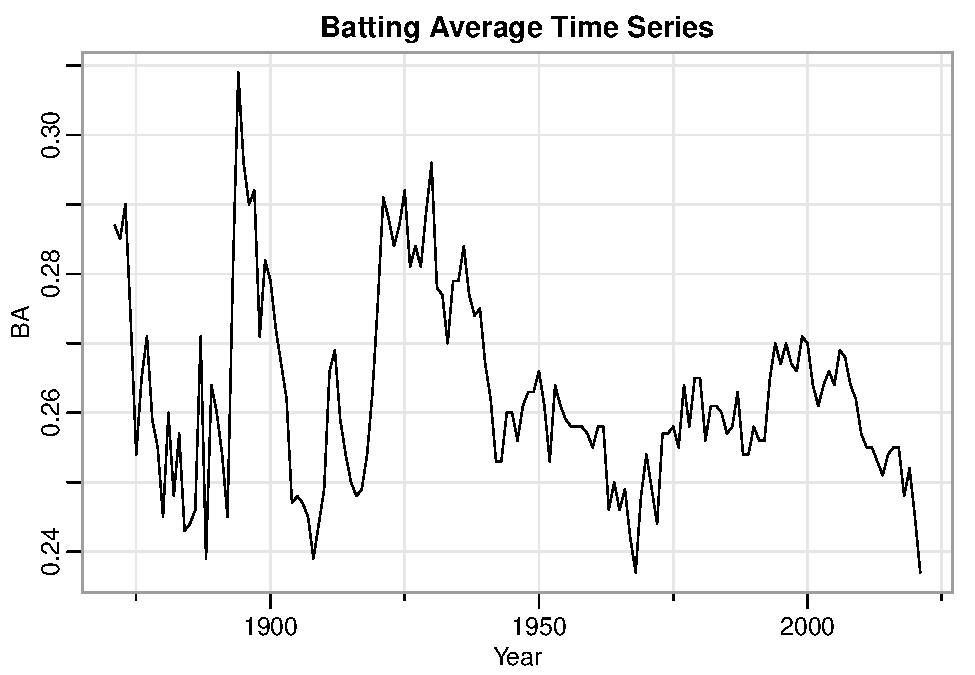
\includegraphics{project_files/figure-latex/unnamed-chunk-2-1.pdf}

\begin{Shaded}
\begin{Highlighting}[]
\NormalTok{hits <-}\StringTok{ }\KeywordTok{ts}\NormalTok{(}\KeywordTok{rev}\NormalTok{(raw}\OperatorTok{$}\NormalTok{H), }\DataTypeTok{start =}\NormalTok{ raw}\OperatorTok{$}\NormalTok{Year[}\KeywordTok{length}\NormalTok{(raw}\OperatorTok{$}\NormalTok{Year)], }\DataTypeTok{end =}\NormalTok{ raw}\OperatorTok{$}\NormalTok{Year[}\DecValTok{1}\NormalTok{])}
\KeywordTok{tsplot}\NormalTok{(hits, }\DataTypeTok{main =} \StringTok{'Hits Time Series'}\NormalTok{, }\DataTypeTok{xlab =} \StringTok{'Year'}\NormalTok{, }\DataTypeTok{ylab =} \StringTok{'Hits'}\NormalTok{)}
\end{Highlighting}
\end{Shaded}

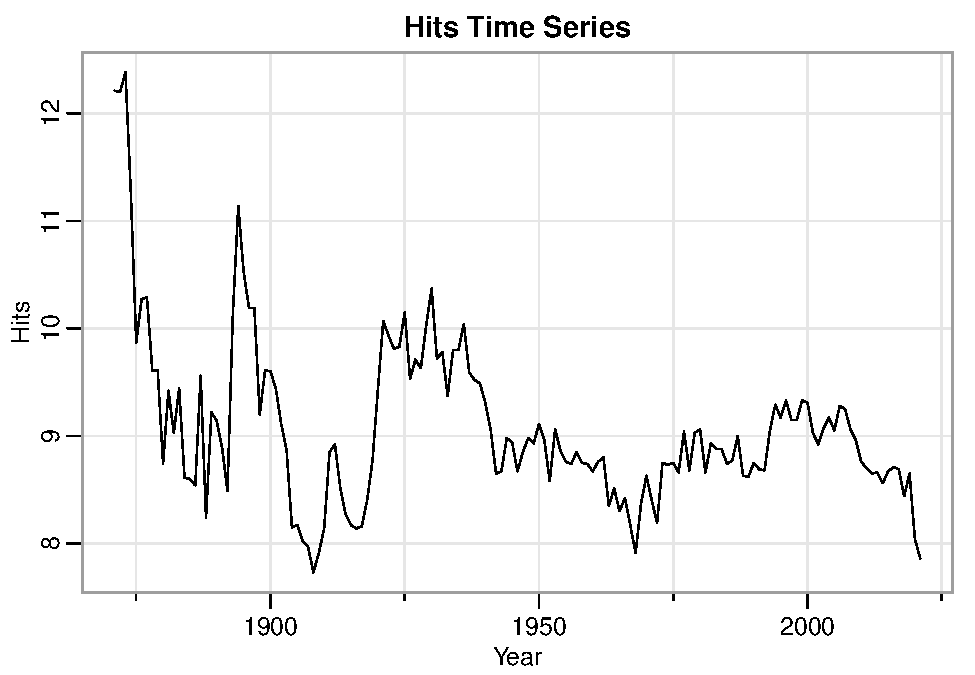
\includegraphics{project_files/figure-latex/unnamed-chunk-3-1.pdf}

\begin{Shaded}
\begin{Highlighting}[]
\NormalTok{hrs <-}\StringTok{ }\KeywordTok{ts}\NormalTok{(}\KeywordTok{rev}\NormalTok{(raw}\OperatorTok{$}\NormalTok{HR), }\DataTypeTok{start =}\NormalTok{ raw}\OperatorTok{$}\NormalTok{Year[}\KeywordTok{length}\NormalTok{(raw}\OperatorTok{$}\NormalTok{Year)], }\DataTypeTok{end =}\NormalTok{ raw}\OperatorTok{$}\NormalTok{Year[}\DecValTok{1}\NormalTok{])}
\KeywordTok{tsplot}\NormalTok{(hrs, }\DataTypeTok{main =} \StringTok{'Home Runs Time Series'}\NormalTok{, }\DataTypeTok{xlab =} \StringTok{'Year'}\NormalTok{, }\DataTypeTok{ylab =} \StringTok{'HRs'}\NormalTok{)}
\end{Highlighting}
\end{Shaded}

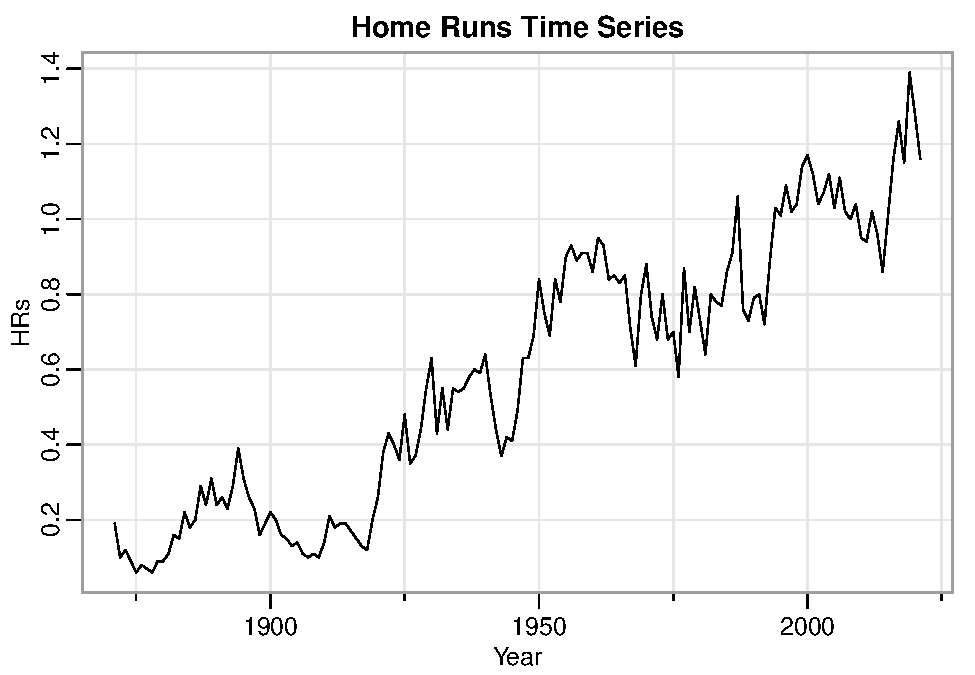
\includegraphics{project_files/figure-latex/unnamed-chunk-4-1.pdf}

\begin{Shaded}
\begin{Highlighting}[]
\NormalTok{so <-}\StringTok{ }\KeywordTok{ts}\NormalTok{(}\KeywordTok{rev}\NormalTok{(raw}\OperatorTok{$}\NormalTok{SO), }\DataTypeTok{start =}\NormalTok{ raw}\OperatorTok{$}\NormalTok{Year[}\KeywordTok{length}\NormalTok{(raw}\OperatorTok{$}\NormalTok{Year)], }\DataTypeTok{end =}\NormalTok{ raw}\OperatorTok{$}\NormalTok{Year[}\DecValTok{1}\NormalTok{])}
\KeywordTok{tsplot}\NormalTok{(so, }\DataTypeTok{main =} \StringTok{'Strikeouts Time Series'}\NormalTok{, }\DataTypeTok{xlab =} \StringTok{'Year'}\NormalTok{, }\DataTypeTok{ylab =} \StringTok{'SOs'}\NormalTok{)}
\end{Highlighting}
\end{Shaded}

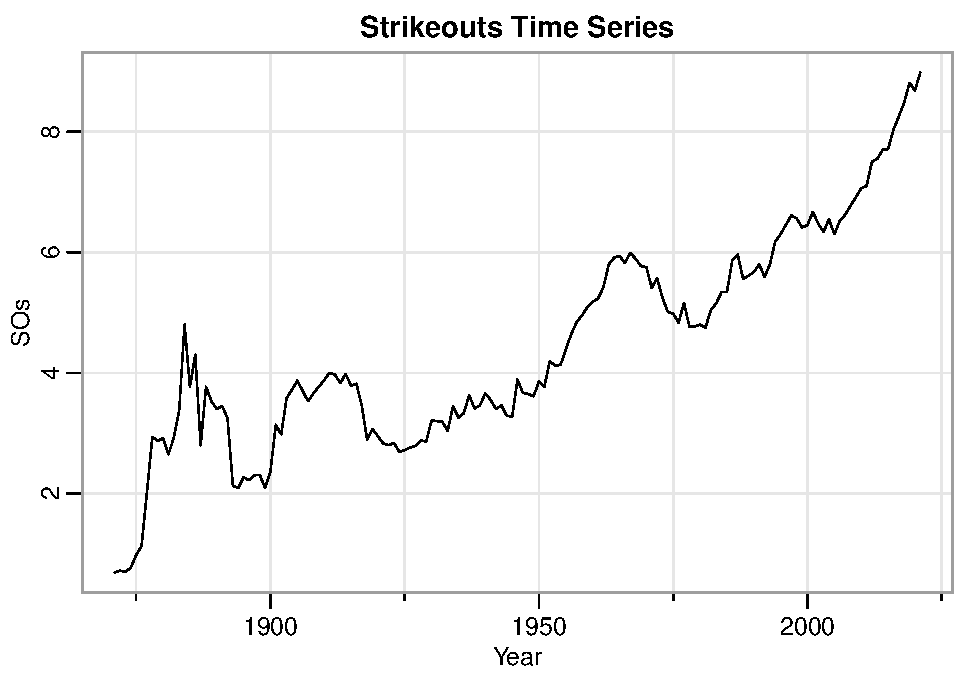
\includegraphics{project_files/figure-latex/unnamed-chunk-5-1.pdf}

\begin{Shaded}
\begin{Highlighting}[]
\NormalTok{panel.cor <-}\StringTok{ }\ControlFlowTok{function}\NormalTok{(x, y, ...) \{}
\NormalTok{  usr <-}\StringTok{ }\KeywordTok{par}\NormalTok{(}\StringTok{"usr"}\NormalTok{); }\KeywordTok{on.exit}\NormalTok{(}\KeywordTok{par}\NormalTok{(usr))}
  \KeywordTok{par}\NormalTok{(}\DataTypeTok{usr =} \KeywordTok{c}\NormalTok{(}\DecValTok{0}\NormalTok{, }\DecValTok{1}\NormalTok{, }\DecValTok{0}\NormalTok{, }\DecValTok{1}\NormalTok{))}
\NormalTok{  r <-}\StringTok{ }\KeywordTok{round}\NormalTok{(}\KeywordTok{cor}\NormalTok{(x, y), }\DecValTok{2}\NormalTok{)}
  \KeywordTok{text}\NormalTok{(}\FloatTok{0.5}\NormalTok{, }\FloatTok{0.5}\NormalTok{, r, }\DataTypeTok{cex =} \FloatTok{1.75}\NormalTok{)}
\NormalTok{\}}
\KeywordTok{pairs}\NormalTok{(}\KeywordTok{cbind}\NormalTok{(}\DataTypeTok{ERA =}\NormalTok{ era, }\DataTypeTok{BattingAvg =}\NormalTok{ ba, }\DataTypeTok{Hits =}\NormalTok{ hits, }\DataTypeTok{Strikeouts =}\NormalTok{ so, }\DataTypeTok{HomeRuns =}\NormalTok{ hrs), }\DataTypeTok{lower.panel =}\NormalTok{ panel.cor)}
\end{Highlighting}
\end{Shaded}

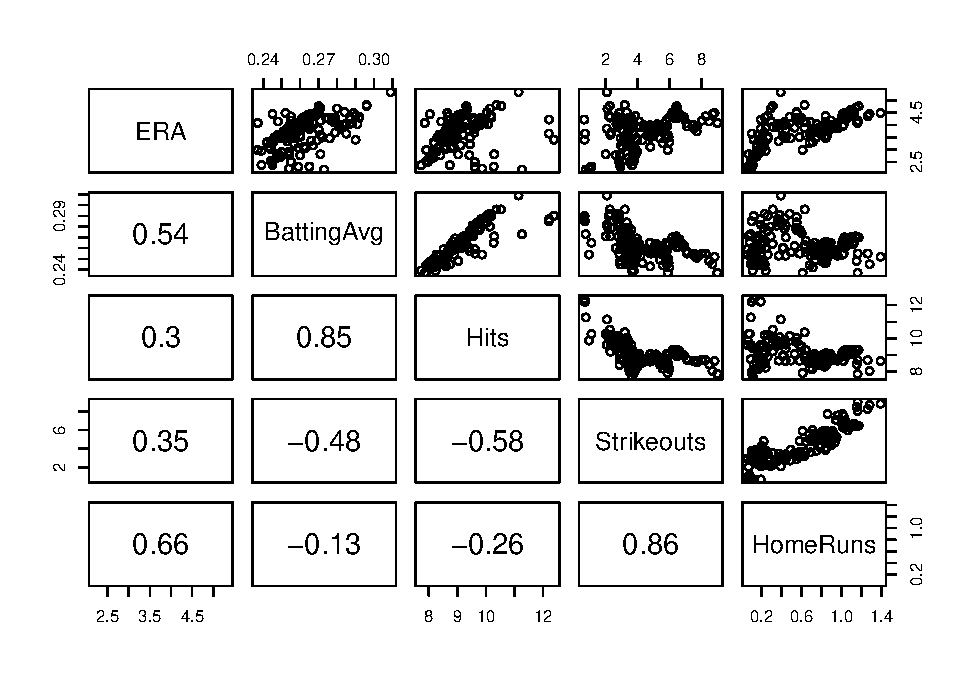
\includegraphics{project_files/figure-latex/unnamed-chunk-6-1.pdf}

\begin{Shaded}
\begin{Highlighting}[]
\KeywordTok{pairs}\NormalTok{(}\KeywordTok{cbind}\NormalTok{(}\DataTypeTok{ERA =}\NormalTok{ era, }\DataTypeTok{BattingAvg =}\NormalTok{ ba, }\DataTypeTok{HomeRuns =}\NormalTok{ hrs), }\DataTypeTok{lower.panel =}\NormalTok{ panel.cor)}
\end{Highlighting}
\end{Shaded}

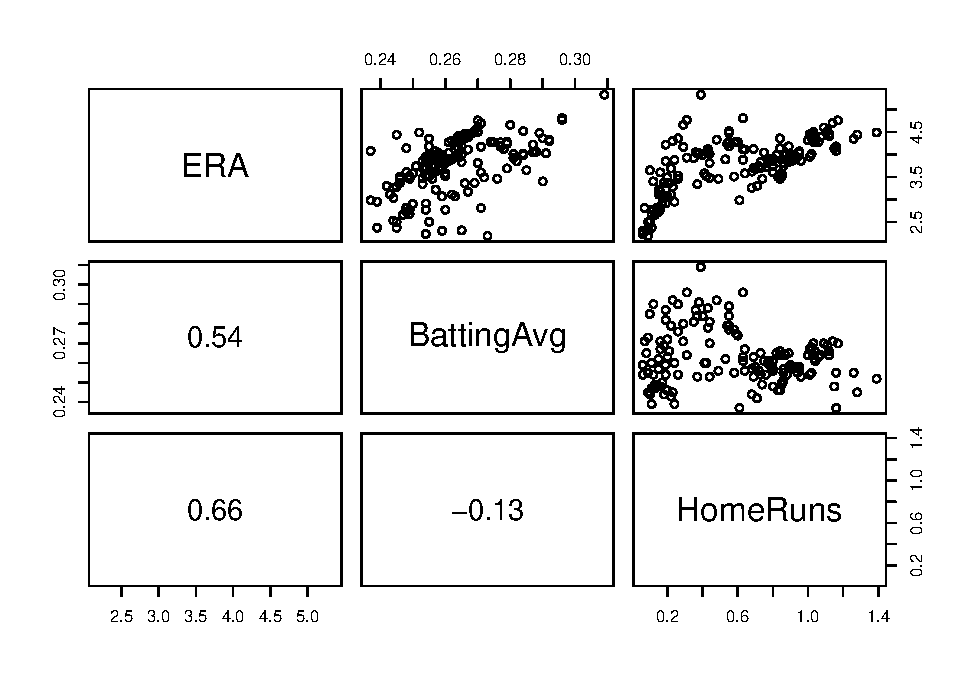
\includegraphics{project_files/figure-latex/unnamed-chunk-7-1.pdf} a.
\(ERA_t = \beta_0 + \beta_1 t + w_t\)\\
b. \(ERA_t = \beta_0 + \beta_1 t + \beta_2 HR + w_t\)\\
c.~\(ERA_t = \beta_0 + \beta_1 t + \beta_2 HR + \beta_3 HR^2 + w_t\)\\
d.~\(ERA_t = \beta_0 + \beta_1 t + \beta_2 HR + \beta_3 HR^2 + \beta_4 BA + w_t\)

\end{document}
